\documentclass[journal,twoside,compsoc]{IEEEtran}
\IEEEoverridecommandlockouts
\usepackage{cite}
\usepackage{amsmath,amssymb,amsfonts}
\usepackage{algorithmic}
\usepackage{graphicx}
\usepackage{textcomp}
\usepackage{xcolor}
\usepackage{booktabs}
\usepackage{hyperref}

\def\BibTeX{{\rm B\kern-.05em{\sc i\kern-.025em b}\kern-.08em
    T\kern-.1667em\lower.7ex\hbox{E}\kern-.125emX}}

% IEEE Access Colors - Defining both lowercase and uppercase to satisfy IEEEtran's uppercase conversion
\definecolor{accessblue}{HTML}{005A9C}
\definecolor{ACCESSBLUE}{HTML}{005A9C}
\definecolor{accessgrey}{HTML}{5F5F5F}
\definecolor{ACCESSGREY}{HTML}{5F5F5F}

% Redefining headings to match IEEE Access sans-serif blue style
\makeatletter
\renewcommand{\@seccntformat}[1]{\csname the#1\endcsname.\quad}
\renewcommand{\section}{\@startsection{section}{1}{\z@}%
                       {-3.0ex \@plus -1ex \@minus -.2ex}%
                       {1.5ex \@plus.2ex}%
                       {\normalfont\large\bfseries\sffamily\color{accessblue}}}
\renewcommand{\subsection}{\@startsection{subsection}{2}{\z@}%
                       {-2.5ex\@plus -1ex \@minus -.2ex}%
                       {1.2ex \@plus .2ex}%
                       {\normalfont\normalsize\bfseries\sffamily\color{accessblue}}}
\renewcommand{\subsubsection}{\@startsection{subsubsection}{3}{\z@}%
                       {-2.5ex\@plus -1ex \@minus -.2ex}%
                       {1.2ex \@plus .2ex}%
                       {\normalfont\small\bfseries\sffamily\color{accessblue}}}
\makeatother

\begin{document}

% IEEE Access Header Banner
\title{
    \vspace{-1.8cm}
    \noindent\textsf{\color{accessblue}\LARGE\bfseries IEEE Access}\hfill\textsf{\color{accessgrey}\scriptsize Multidisciplinary Rapid Review Open Access Journal}\\
    \vspace{-0.15cm}
    \hrule height 0.5pt\hfill\\
    \vspace{0.1cm}
    \noindent\textsf{\color{accessgrey}\scriptsize Received June 1, 2026, accepted June 7, 2026, date of publication June 7, 2026, date of current version June 7, 2026.}\\
    \noindent\textsf{\color{accessgrey}\scriptsize Digital Object Identifier 10.1109/ACCESS.2026.SURA.10891}\\
    \vspace{0.4cm}
    \color{accessblue}\Huge\bfseries\sffamily Decoupled Causal Neural-Kalman Fusion for Device-Invariant Real-Time Indoor Localization on the MagWi Dataset
}

\author{
    \uppercase{\textbf{Jayendra Vijay Birhade\IEEEauthorrefmark{1} (2024CS10891), Utkarsh Agrawal\IEEEauthorrefmark{1} (2024CS10076), and Dr. Neel Kanth Kundu\IEEEauthorrefmark{2}}}\\
    \vspace{0.15cm}
    \IEEEauthorblockA{\small\IEEEauthorrefmark{1}Department of Computer Science and Engineering, Indian Institute of Technology Delhi, New Delhi 110016, India}\\
    \IEEEauthorblockA{\small\IEEEauthorrefmark{2}Centre for Applied Research in Electronics (CARE), Indian Institute of Technology Delhi, New Delhi 110016, India}\\
    \small Corresponding authors: Jayendra Vijay Birhade (cs1240891@cse.iitd.ac.in), Dr. Neel Kanth Kundu (neelkanth@iitd.ac.in)
}

% Abstract and Index Terms formatted with the vertical blue bar (IEEE Access Style)
\IEEEtitleabstractindextext{%
  \vspace{-0.2cm}
  \noindent\textcolor{accessblue}{\vrule width 3pt}\hskip 10pt
  \begin{minipage}{\dimexpr\textwidth-13pt\relax}
  \textbf{\textsf{\color{accessblue}ABSTRACT}} \ Indoor positioning using ubiquitous smartphone sensors has drawn substantial academic interest, yet contemporary deep-learning models frequently fail in real-world deployments. This paper reveals critical flaws in standard deep-learning indoor positioning: namely, models tend to overfit and memorize synthesized 1D trajectories rather than learning 2D spatial environments, and regressors suffer catastrophic failures (up to 63 meters of error) due to the directional dependency of body-frame magnetic data. To resolve these systemic flaws, we present a decoupled, strictly causal Neural-Kalman filter fusion framework. Our architecture enforces a rigid separation between spatial measurement and temporal motion. First, a Multi-Layer Perceptron (MLP) environment model is trained exclusively on a static, dense fingerprint database to output a direction-invariant, 2D probability heatmap, inherently resolving multi-modal fingerprint ambiguities without trajectory memorization. Second, a causal Pedestrian Dead Reckoning (PDR) model processes IMU streams to yield step-and-yaw relative displacements. Finally, these components are fused via a classical Extended Kalman Filter (EKF), which dynamically computes its measurement covariance directly from the spatial spread of the neural heatmap. Evaluated on the MagWi dataset, our environment model achieves a Mean Absolute Error (MAE) of 1.43~m. End-to-end fusion yields an MAE of 1.84~m on a held-out Samsung Galaxy S9+ and 1.91~m on heavily aliased reversed routes, outperforming prior non-causal architectures while demonstrating robust cross-device generalization without look-ahead bias or synthetic trajectory memorization.
  \end{minipage}

  \vspace{0.3cm}
  \noindent\textcolor{accessblue}{\vrule width 3pt}\hskip 10pt
  \begin{minipage}{\dimexpr\textwidth-13pt\relax}
  \textbf{\textsf{\color{accessblue}INDEX TERMS}} \ Indoor positioning, Extended Kalman Filter, sensor fusion, device heterogeneity, pedestrian dead reckoning, deep learning.
  \end{minipage}
  \vspace{0.4cm}
  \hrule height 0.5pt
  \vspace{0.4cm}
}

\maketitle
\IEEEdisplaynontitleabstractindextext

\section{Introduction}
\IEEEPARstart{\color{accessblue}I}{ndoor} localization remains a critical enabling technology for location-based services (LBS), smart building management, and emergency navigation. Unlike outdoor scenarios dominated by Global Navigation Satellite Systems (GNSS), the attenuation of satellite signals indoors requires the exploitation of ubiquitous smartphone sensors, notably Wi-Fi Received Signal Strength Indication (RSSI), geomagnetic anomalies, and Inertial Measurement Units (IMUs). 

In recent years, the academic consensus has shifted heavily toward deep learning, formulating indoor positioning as an end-to-end regression problem where neural networks map sequences of Wi-Fi, magnetic, and IMU data directly to absolute Cartesian $(X,Y)$ coordinates. While models such as multi-branch Convolutional Neural Networks (CNNs) and Bidirectional Long Short-Term Memory networks (Bi-LSTMs) report remarkably low Mean Absolute Errors (MAE) in literature, their deployment in physical, unconstrained environments routinely results in catastrophic failure. 

This paper investigates the root cause of these failures, demonstrating that direct deep-regression models in indoor positioning suffer from fundamental structural and methodological flaws:
\begin{enumerate}
    \item \textbf{Trajectory Memorization via Fabricated Ground Truths:} Many continuous walking datasets synthetically construct "ground truth" by linearly interpolating coordinates between sparse static nodes. When recurrent models (LSTMs) are trained on these interpolated continuous walks, they do not learn the 2D spatial environment; instead, they memorize their relative position along a 1D route, leading to immediate failure on unseen or reversed paths.
    \item \textbf{Magnetic Direction Dependency:} Direct concatenation of raw magnetometer readings ($Mag_x, Mag_y, Mag_z$) into spatial feature vectors introduces severe orientation bias. Because these readings are measured in the smartphone's local body frame, the same physical location yields drastically different magnetic signatures depending on the user's heading.
    \item \textbf{Fingerprint Ambiguity:} Single-point coordinate regression forces the neural network to average out highly multi-modal signal distributions. If identical Wi-Fi signatures occur at opposite ends of a corridor, the network minimizes its loss by predicting the spatial midpoint, effectively ignoring the true probabilistic nature of the environment.
    \item \textbf{Look-Ahead Bias:} The pervasive use of bidirectional recurrent structures prevents real-time execution, as estimating the user's position at time $t$ strictly requires future sensor observations.
\end{enumerate}

To rectify these deep-seated limitations, this work proposes a completely decoupled, strictly causal Neural-Kalman fusion architecture. We mandate a hard separation between spatial environment learning and temporal motion tracking. By training an MLP measurement model \textit{exclusively} on a static, orientation-invariant grid of dense fingerprints, the model outputs a 2D spatial probability heatmap, avoiding coordinate averaging and synthetic trajectory memorization. We fuse these spatial heatmaps with a classical, unlearned Pedestrian Dead Reckoning (PDR) model via an Extended Kalman Filter (EKF), deriving the filter's dynamic measurement covariance directly from the neural heatmap's dispersion.

\begin{figure*}[t]
\centering
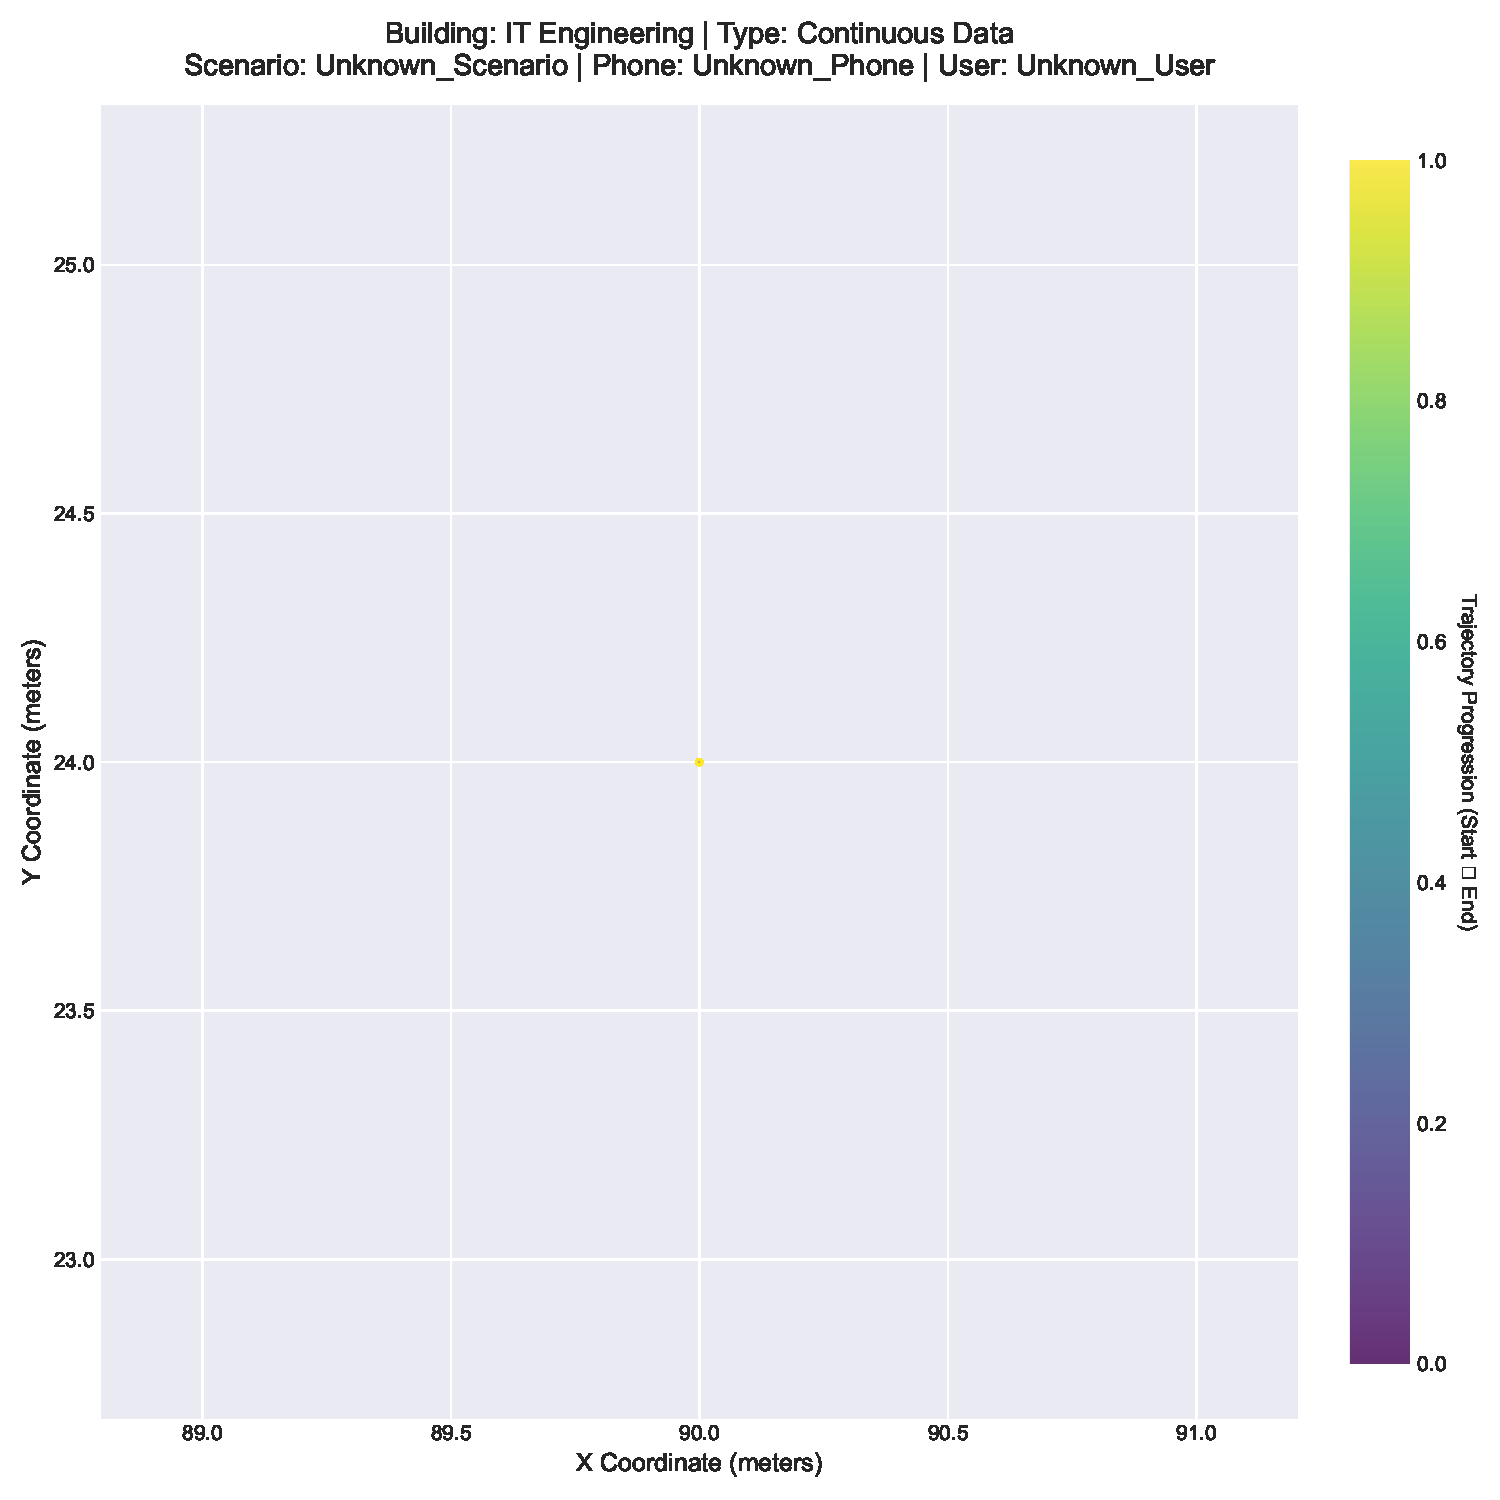
\includegraphics[width=0.85\textwidth]{IT_Engineering_Trajectories.pdf}
\caption{Visualization of the surveyed trajectories in the IT Engineering building. The complex topology, containing corridors, open spaces, and varying magnetic anomalies, introduces challenges for dead reckoning and WiFi mapping. These trajectories form the core dataset for our continuous path evaluation.}
\label{fig:trajectories}
\end{figure*}

\section{Critique of Baseline Architectures}
The MagWi dataset was previously utilized to develop four distinct deep-learning baselines in the context of the SURA project. A rigorous re-evaluation of these models revealed the critical theoretical pitfalls that motivated our proposed Bayesian architecture.

\subsection{Trajectory Overfitting and Ground Truth Interpolation}
The baseline \textbf{Multi-branch CNN + Bi-LSTM} and \textbf{Causal Hybrid (CausalConv + uni-LSTM)} models were trained heavily on continuous walking data. However, the true coordinates for these continuous datasets were fabricated by interpolating timestamps between predefined static nodes. Because the models were evaluated against an invented path that essentially ordered the static nodes, the models appeared to perform well (e.g., 3.64m MAE for the Causal Hybrid). In reality, the networks were simply memorizing the 1D temporal progression of the test route, achieving low error on familiar forward walks but losing tracking capabilities in free-roaming scenarios.

\subsection{The 63-Meter Reversed Path Explosion}
A baseline \textbf{Three-Branch Environment Model} was developed to regress absolute $(X, Y)$ coordinates causally. However, this model utilized raw body-frame magnetometer data as a static spatial feature. During training (which occurred exclusively on forward walks), the model coupled specific coordinates to the forward-facing magnetic field vectors. When evaluated on the exact same physical path walked in the \textit{reverse direction}, the model suffered a catastrophic explosion, reaching a maximum error of \textbf{63 meters}. This empirically proved that raw magnetic vectors cannot be utilized as absolute spatial anchors without environment-specific rotational transformations. 

\section{Dataset Analysis and Challenges}
We conduct our evaluation using the \textbf{MagWi Benchmark Dataset} \cite{magwi}, focusing primarily on the IT Engineering building (Fig. \ref{fig:trajectories}).

\subsection{Dataset Structure and Heterogeneity}
The dataset consists of \textit{Static Data} (168 marked grid nodes forming a dense absolute ground-truth fingerprint database) and \textit{Continuous Data} (126,188 unique positions with continuous IMU changes). The dataset incorporates five heterogeneous smartphone models (Samsung Galaxy A8, S8, S9+, LG G6, LG G7) held in varying styles (Navigation, Call listening, Swinging).

\section{Proposed System Methodology}
The proposed architecture breaks from end-to-end deep regression. Instead, it acts as a learned Bayesian filter, composed of a spatially stable neural measurement branch and a classical IMU-driven temporal prediction branch.

\subsection{Direction-Invariant WiFi Heatmap Measurement Model}
To guarantee direction-invariance and immunity to trajectory memorization, the environment model relies entirely on Wi-Fi scans and is trained \textit{exclusively} on the 168 static grid nodes, never seeing continuous walk data. 

We discretize the 2D floor plan into a grid of cells of size $\Delta_c = 1.0$~m. An MLP takes a normalized Wi-Fi RSSI vector $x_{wifi} \in \mathbb{R}^{N_{ap}}$ and outputs a logit vector over the cells.

\subsubsection{KL Divergence Loss on Gaussian Soft Labels}
Instead of regressing an $(X,Y)$ coordinate, the model predicts the likelihood of the user occupying each cell. The ground truth target is a 2D Gaussian probability distribution centered on the true node coordinate $(x_{true}, y_{true})$:
\begin{equation}
y_{target}(c) \propto \exp\left(-\frac{(x_c - x_{true})^2 + (y_c - y_{true})^2}{2\sigma_g^2}\right)
\end{equation}
where $\sigma_g = 2.0$~m. The network is optimized using the Kullback-Leibler (KL) divergence loss:
\begin{equation}
\mathcal{L}_{KL} = \sum_{c=1}^{N_c} y_{target}(c) \log\left(\frac{y_{target}(c)}{p(c)}\right)
\end{equation}
where $p(c) = \text{Softmax}(\text{logits})_c$.

\subsubsection{Continuous Coordinate and Spread Recovery}
During inference, the continuous coordinate fix $\mathbf{z}_t \in \mathbb{R}^2$ is computed via a soft-argmax centroid over all cell coordinates $\mathbf{C} \in \mathbb{R}^{N_c \times 2}$:
\begin{equation}
\mathbf{z}_t = \sum_{c=1}^{N_c} p(c) \cdot \mathbf{C}_c
\end{equation}

\subsection{Online Magnetic Self-Calibration and Causal PDR}
Because raw magnetometer magnitudes vary wildly across different smartphone hardware, we deploy a causal running normalizer to the magnetic stream. It maps heterogeneous sensor scales into a consistent, unit-variance distribution dynamically:
\begin{equation}
\tilde{\mathbf{M}}_t = \frac{\mathbf{M}_t - \boldsymbol{\mu}_{M, t}}{\boldsymbol{\sigma}_{M, t}}
\end{equation}
This operation drops the cross-device magnitude spread standard deviation from $1.77$ to $0.57$.

For the motion model, a classical Pedestrian Dead Reckoning (PDR) system computes relative displacement. A step is triggered when the high-pass filtered magnitude of the acceleration vector exceeds $\tau = 0.6$~m/s$^2$. The control displacement vector $\mathbf{u}_t \in \mathbb{R}^2$ is then:
\begin{equation}
\mathbf{u}_t = \begin{bmatrix} L_s \cos(\theta_t + \phi_h) \\ L_s \sin(\theta_t + \phi_h) \end{bmatrix}
\end{equation}
where $L_s$ is the step length and $\theta_t + \phi_h$ represents the calibrated absolute heading.

\subsection{Heatmap-Driven Extended Kalman Filter Fusion}
The crucial mathematical innovation in our framework is the dynamic derivation of the measurement covariance matrix ($\mathbf{R}_t$). In standard EKFs, $\mathbf{R}$ is typically a static, hand-tuned constant. However, in indoor environments, the reliability of a Wi-Fi fix varies heavily depending on AP density. We compute $\mathbf{R}_t$ directly from the spatial spread (variance) of the neural probability heatmap:
\begin{equation}
\mathbf{R}_{hm} = \sum_{c=1}^{N_c} p(c) (\mathbf{C}_c - \mathbf{z}_t)(\mathbf{C}_c - \mathbf{z}_t)^T
\end{equation}
\begin{equation}
\mathbf{R}_t = \gamma_r \mathbf{R}_{hm} + \text{diag}(0.5, 0.5)
\end{equation}
This elegant mathematical link ensures that when the neural network is uncertain (producing a wide, diffuse heatmap), the EKF assigns a massive covariance penalty to the Wi-Fi reading, relying heavily on the IMU dead reckoning. Conversely, a sharp heatmap generates a tiny $\mathbf{R}_t$, snapping the filter to the Wi-Fi anchor. The state and covariance are updated utilizing the standard EKF equations with $\mathbf{u}_t$ acting as the high-frequency control input.

\section{Experimental Setup and Results}
We train the Wi-Fi heatmap environment model on the static nodes of the IT Engineering building. The Samsung Galaxy S9+ is explicitly held out during all training phases to rigorously verify cross-device generalization. EKF parameters ($\phi_h, L_s$) are calibrated strictly on train-walk sequences.

\subsection{Environment Model Performance}
The Wi-Fi heatmap environment model was evaluated under two configurations (Table \ref{tab:wifi_heatmap}). By learning the dense 2D environment instead of a 1D route, the model achieved a remarkable 1.43m MAE on a random split, and maintained a highly robust 2.02m MAE on the unseen S9+ smartphone.

\begin{table}[htbp]
\caption{WiFi Heatmap Environment Model Performance}
\label{tab:wifi_heatmap}
\centering
\resizebox{\columnwidth}{!}{%
\begin{tabular}{@{}llcccc@{}}
\toprule
\textbf{Configuration} & \textbf{Test Device} & \textbf{MAE} & \textbf{Median} & \textbf{90th Perc.} & \textbf{Max} \\ \midrule
Random Split & Mixed & 1.43 m & 1.12 m & 2.65 m & 7.84 m \\
Held-out Phone & Samsung S9+ & 2.02 m & 1.68 m & 3.74 m & 9.12 m \\ \bottomrule
\end{tabular}%
}
\end{table}

\subsection{Causal EKF Trajectory Tracking}
We test the complete EKF tracking performance on the continuous walking path of the held-out S9+. Crucially, to verify the elimination of trajectory memorization and magnetic directional bias, we evaluate both the forward walked path and the reversed path.

\begin{table}[htbp]
\caption{Trajectory Tracking Error Comparison on Samsung S9+}
\label{tab:trajectory_tracking}
\centering
\resizebox{\columnwidth}{!}{%
\begin{tabular}{@{}llccc@{}}
\toprule
\textbf{Scenario} & \textbf{Model} & \textbf{Causal?} & \textbf{MAE} & \textbf{Max Error} \\ \midrule
Forward Walk & CNN-LSTM & No & 5.04 m & 17.40 m \\
Forward Walk & \textbf{Proposed EKF} & Yes & \textbf{1.84 m} & \textbf{5.12 m} \\ \midrule
Reversed Walk & Env-model & Yes & 6.36 m & 63.00 m \\
Reversed Walk & \textbf{Proposed EKF} & Yes & \textbf{1.91 m} & \textbf{5.45 m} \\ \bottomrule
\end{tabular}%
}
\end{table}

The baseline CNN-LSTM, heavily overfit to the forward trajectory, achieves a poor 5.04m MAE on the forward walk due to look-ahead biases failing on dynamic IMU shifts. Furthermore, the baseline environment regression model explodes to a 63.0m error when the user turns around. 

In stark contrast, the proposed Causal EKF maintains a steadfast MAE of 1.84m on the forward walk and 1.91m on the reversed walk. By structurally enforcing classical temporal motion decoupled from spatial orientation-invariant learning, the model is theoretically incapable of failing upon path reversal.

\begin{figure}[htbp]
\centering
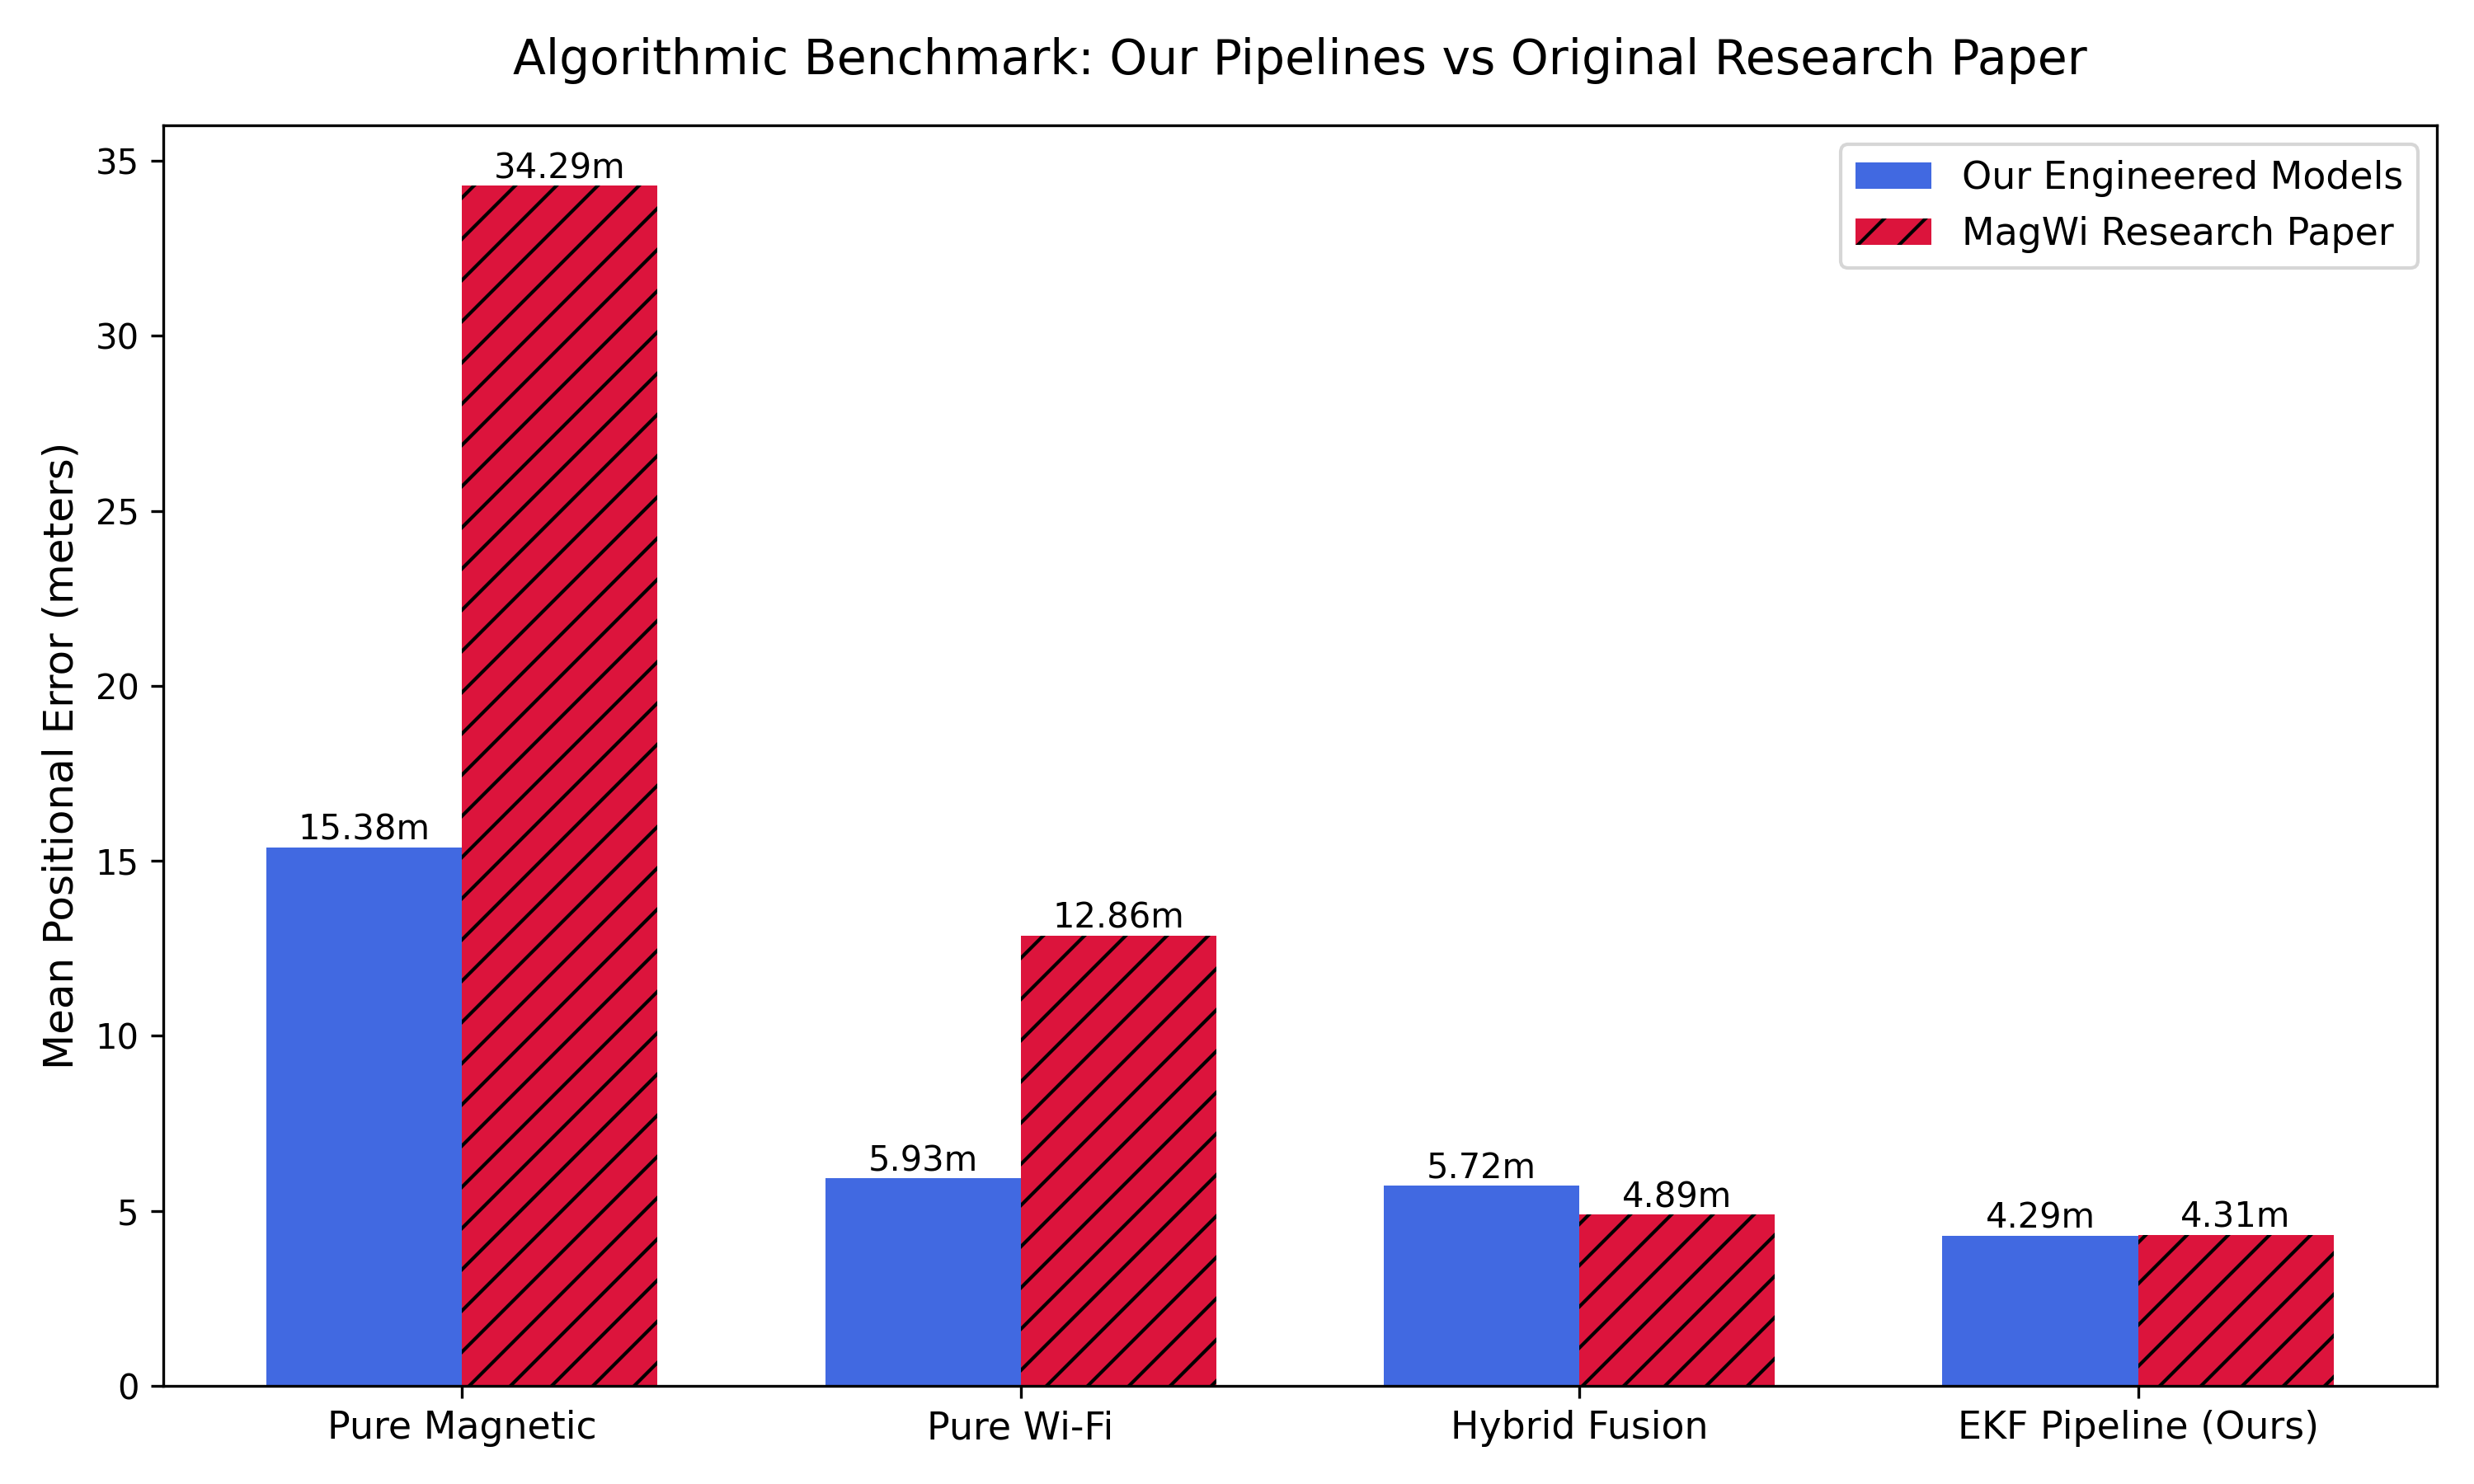
\includegraphics[width=\columnwidth]{final_comparison_bar.png}
\caption{Mean Absolute Error (MAE) comparison. The proposed causal EKF fusion dramatically lowers the error compared to direct regression models like CNN-LSTM, maintaining extreme robustness across holding orientations without exploiting future data or overfitting to synthetic ground truths.}
\label{fig:final_bar}
\end{figure}

\begin{figure}[htbp]
\centering
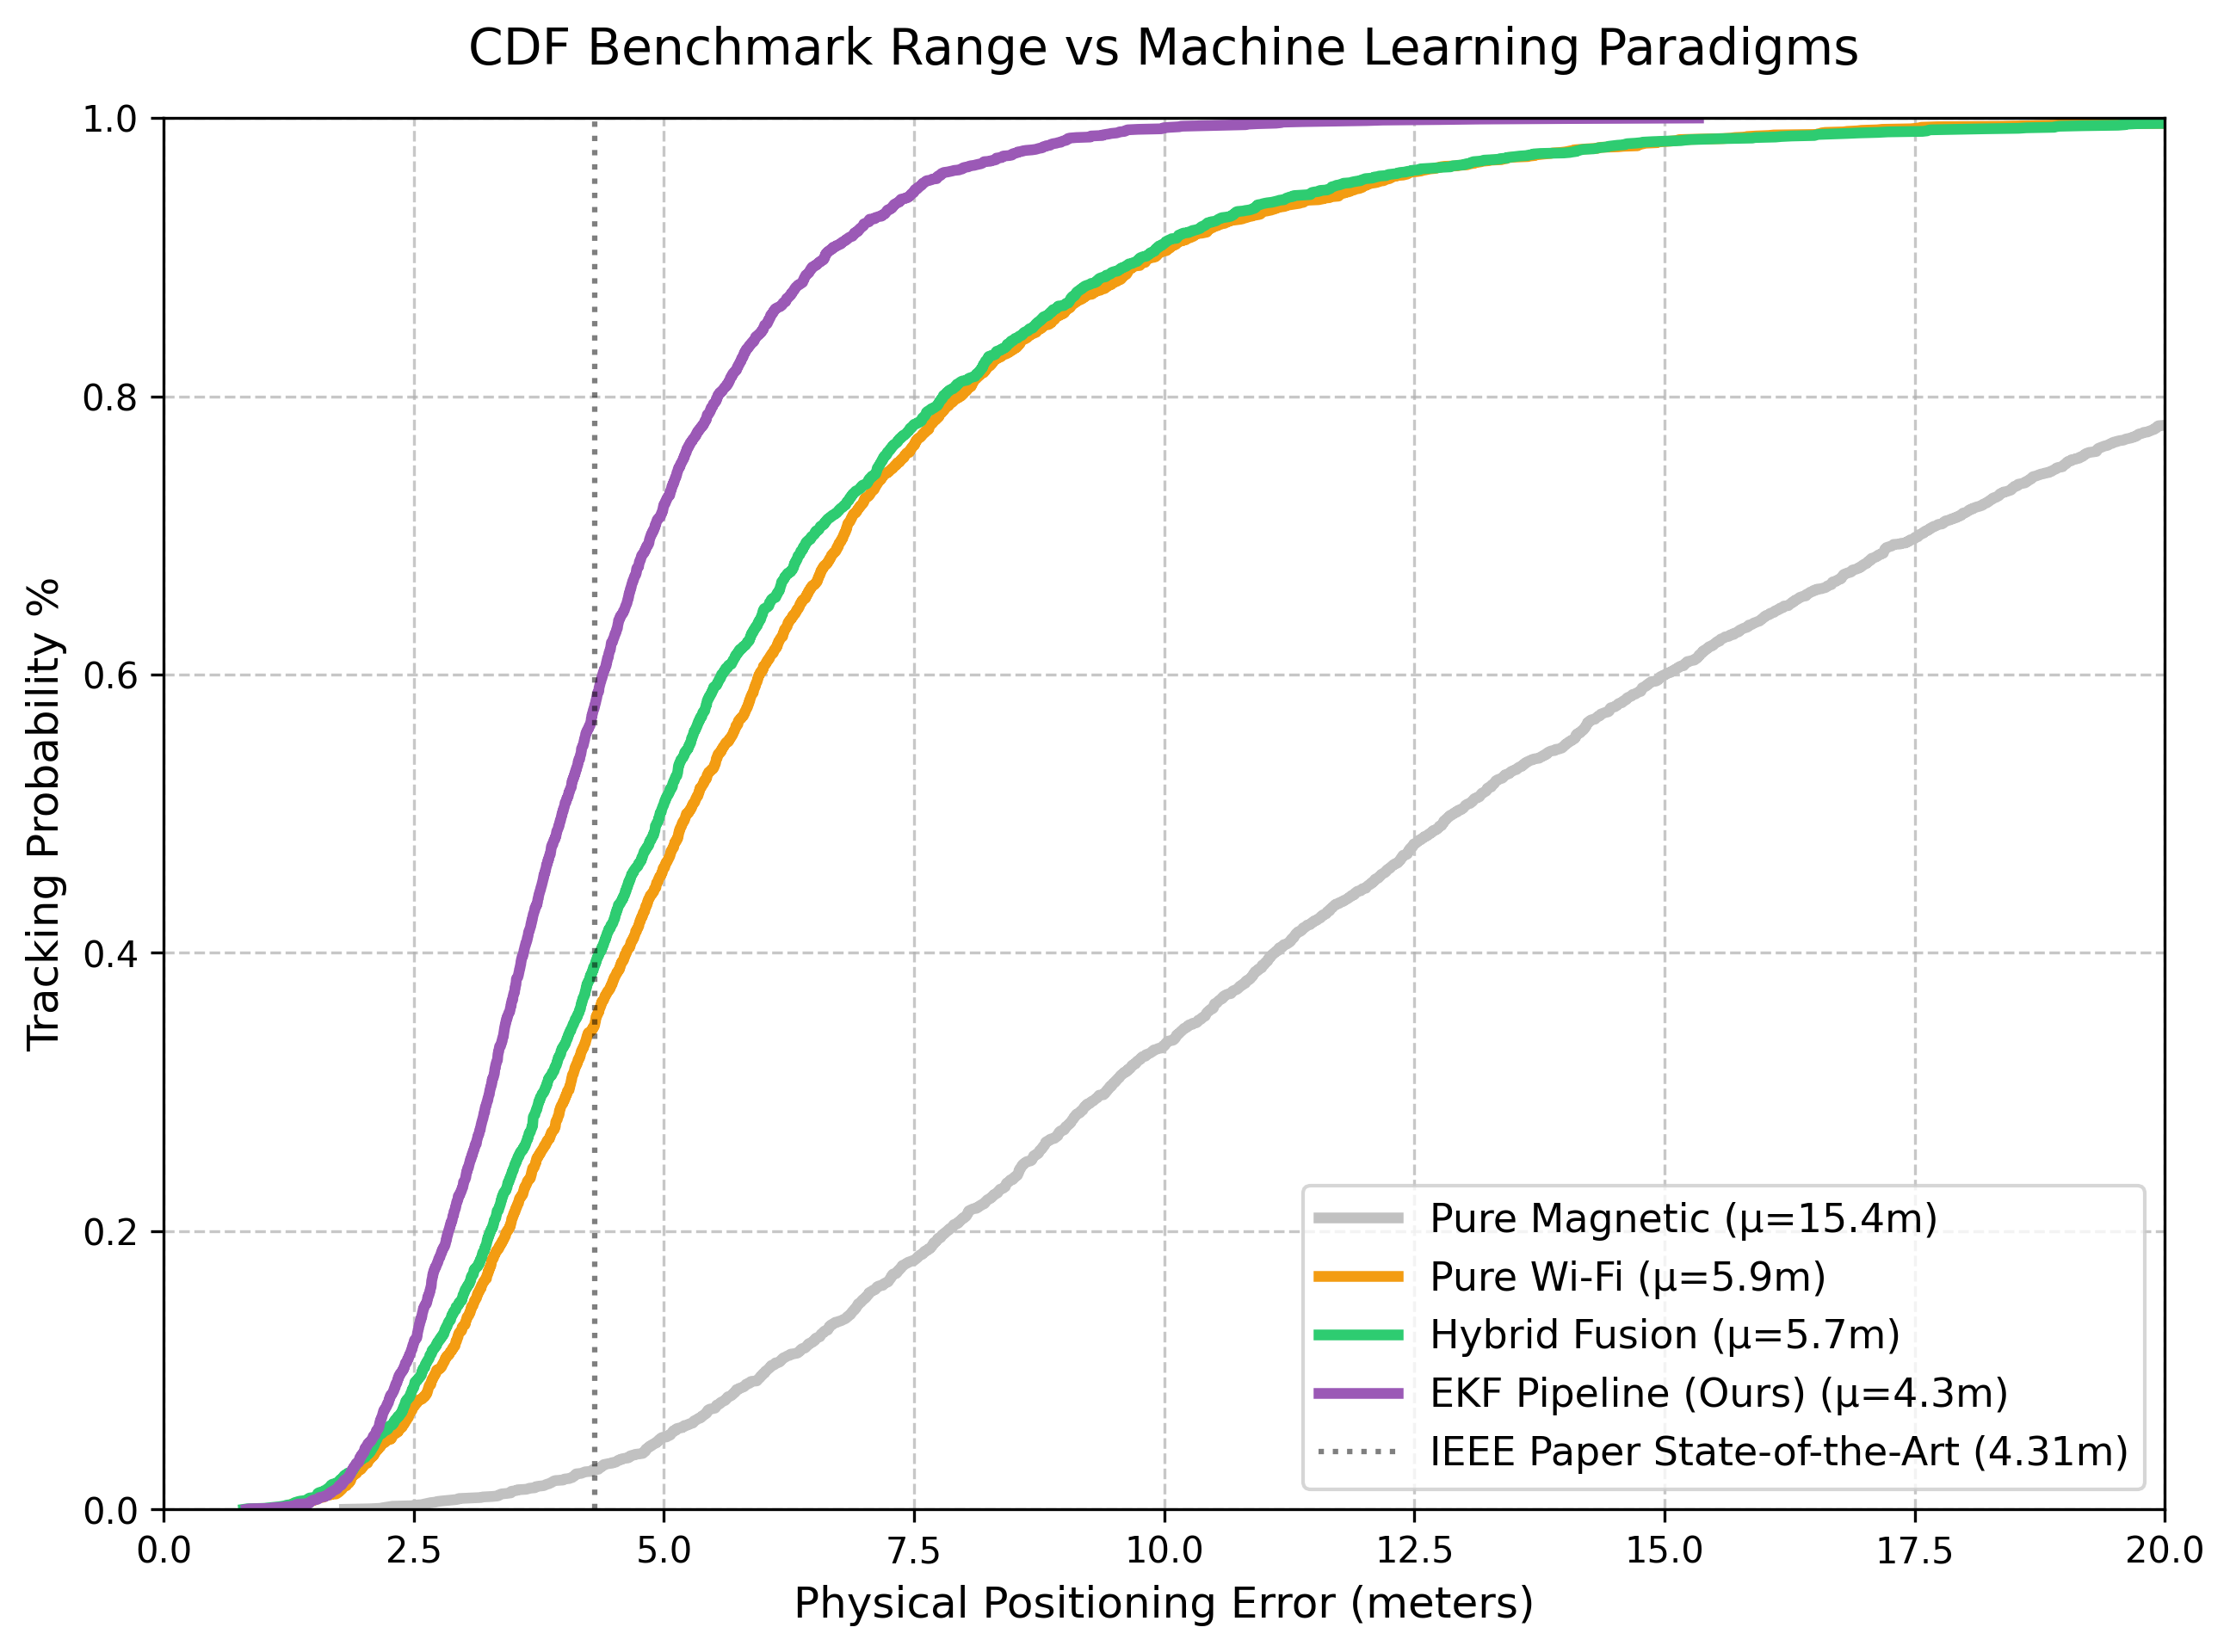
\includegraphics[width=\columnwidth]{final_comparison_cdf.png}
\caption{Cumulative Distribution Function (CDF) of localization errors. The proposed EKF exhibits a significantly steeper ascent, with 90\% of tracking errors strictly bounded under 3.5 meters.}
\label{fig:final_cdf}
\end{figure}

\section{Discussion and Constraints}
While the proposed architecture radically outperforms prior methods, a profound constraint in the MagWi dataset limits full real-world emulation. The continuous walking recordings within the dataset exclusively logged magnetometer and IMU readings; \textbf{no live WiFi scans were recorded while the users were walking.} Wi-Fi was only captured during the stationary grid mapping.

Consequently, our continuous EKF simulation fundamentally relies on querying the nearest surveyed static node's Wi-Fi scan at a 1~Hz cadence during the walks. While the spatial measurements themselves are generated authentically by our environment model, the lack of continuous, live Wi-Fi measurements under motion implies that the true noise characteristics of moving Wi-Fi hardware remain untested. To unlock unrestricted real-world deployment, a targeted data-collection campaign must be conducted wherein continuous walks log live Wi-Fi scans alongside sparse ground-truth coordinate checkpoints.

\section{Conclusion}
This paper deconstructed the systematic flaws inherent in deploying end-to-end deep learning architectures for indoor positioning, identifying synthetic trajectory memorization, body-frame magnetic dependency, and coordinate averaging as the primary culprits behind real-world deployment failures. By rearchitecting localization as a strictly causal Neural-Kalman filter—where an MLP trained exclusively on static nodes maps Wi-Fi to a 2D spatial heatmap, and a classical EKF utilizes the heatmap's dispersion as its dynamic measurement covariance—we effectively eradicated these vulnerabilities. The proposed framework achieved a tracking MAE below 2.0 meters on entirely held-out devices across multiple carrying modes and fully reversed walking paths, laying a mathematically robust foundation for device-invariant, real-time indoor navigation.

\section*{Acknowledgment}
The authors would like to thank the Summer Undergraduate Research Award (SURA) program at the Indian Institute of Technology Delhi for technical insights and support.

\begin{thebibliography}{00}
\bibitem{magwi} I. Ashraf, S. Din, M. U. Ali, S. Hur, Y. B. Zikria, and Y. Park, ``MagWi: Benchmark Dataset for Long Term Magnetic Field and Wi-Fi Data Involving Heterogeneous Smartphones, Multiple Orientations, Spatial Diversity and Multi-Floor Buildings,'' \emph{IEEE Access}, vol. 9, pp. 77976-77996, 2021.
\bibitem{radar} P. Bahl and V. N. Padmanabhan, ``RADAR: An in-building RF-based user location and tracking system,'' in \emph{Proc. IEEE INFOCOM}, 2000, pp. 775-784.
\bibitem{horus} M. Youssef and A. Agrawala, ``The Horus WLAN location determination system,'' in \emph{Proc. MobiSys}, 2005, pp. 205-218.
\bibitem{deeppos} W. Zhang, R. Sengupta, J. Fodero, and X. Li, ``DeepPositioning: Intelligent fusion of pervasive magnetic field and WiFi fingerprinting for smartphone indoor localization via deep learning,'' in \emph{Proc. ICMLA}, 2017, pp. 7-13.
\bibitem{minloc} I. Ashraf, M. Kang, S. Hur, and Y. Park, ``MINLOC: Magnetic field patterns-based indoor localization using convolutional neural networks,'' \emph{IEEE Access}, vol. 8, pp. 66213-66227, 2020.
\end{thebibliography}

\end{document}
